\chapter{Phase 2 Development}
\label{chap:work}

This chapter details the development work that has been performed in the second phrase of the project.  This includes conceptual problems faced and their solutions.

%For each of the below, why, how inc conceptual problems, impact, how it could be improved

\section{Design Decisions}
\label{sec:design}

During this phase of development a number of design decisions had to be made.  The decisions broadly fell into two categories:  \ac{UI} decisions and architectural decisions.  Ideally there should be a method behind such decisions.  The decisions and the reasoning behind them are below.

\subsection{\ac{UI} Design}

During the planning phase of the project (MPP) wireframe designs of the \ac{UI} components were developed.  The purpose of these wireframes was to allow for the \ac{UI} to be evaluated, at least once, before development started.  It is cheaper to fix problems early. Fixing the problem before any development is particularly cheap.

The previous wireframe evaluation that was performed was useful, but not for evaluating the \ac{UI}.  The main insights from the wireframe evaluation were to do with potential functionality.  Very little was learned about the user's thoughts on potential \acp{UI}.  The insights into functionality could be learned without the wireframes being mocked up.  This is what happened in the evaluations during this phase of development.

During the second phase of development (MPP2) the \ac{UI} was refined and new elements were added to it.  It would have been desirable to again first create wireframes and evaluate them with the users before starting development.  This approach was not feasible in this stage of development.  It would have been necessary to hold more frequent user evaluations, which would have placed a greater strain on the user's time.  The alternative would have been to keep the evaluations at the planned frequency and have the development bottlenecked by evaluating the wireframes.  It was decided to not use wireframe prototypes. Instead the \ac{UI} was developed and then users evaluated it.  The \ac{UI} was then changed as required.  The improvement of the architecture outlined in Section~\ref{sec:architecture} made changes to the \ac{UI} easier.  After the improvement the \ac{UI} contained much less information about the state of the tool.  The \ac{UI} is now effectively just calling the \ac{API}.  Having the \ac{UI} separated means that a change to the \ac{UI} no longer requires a refactoring of program logic.

\subsection{Architectural Design}
\label{sec:architecture}
After the first stage of development there was little architectural design.  The three main elements of the tool were the \ac{UI}, the graph visualisation, and the model visualisation.  Each component of the \ac{UI} contained different parts of the visualisation data.  Some parts of this data were duplicated across different parts of the program.   As you can see in Figure~\ref{fig:initial_architecture} each component was passing information to the other components.  Some of the items being passed around had references to to other components.  At the start of this phase of development (MPP2) the features that were to be implemented were too complex for this `lack of architecture' architecture.

The program was refactored to focus on an architectural model where all the data was centralised in a single location.  This can be seen in Figure~\ref{fig:final_architecture}.  If the original architecture was continued, with the new components included, the interaction would look like Figure~\ref{fig:initial_architecture_future}.  Trying to debug and add additional features would have been non trivial.  The visualisation and \ac{UI} components select what they need to display from this central location.  The simplified architecture in Figure~\ref{fig:final_architecture} greatly reduced the amount of information that was having to be passed between all the components.  A refresh of the \ac{UI} components is then all that is needed to display the most up to date information.  This is similar to the \ac{MVC} architecture.  A simple diagram for \ac{MVC} can be seen in Figure~\ref{fig:mvc}.  In this case the controller and the view are not entirely separated.  The model in this project is the session state that contains the information to be displayed.  The distinction between the view and the controller is currently blurred with some aspect of control being handled by the view.  Separating these would be a priority for future work.

A singleton was used to store the session state.  A singleton only allows one instance of itself.  This prevented the accidental creation of multiple session state objects.  Using a singleton helped guaranteed that all session data would be kept together.

This work to move all the session data to being in a centralised location also enabled two new features: undo/redo, and saving and loading.

\paragraph*{Undo and Redo} is implemented by pushing and popping copies of this session state onto a stack.  The copy of the session data that we want to display is the head of the stack.  Undo and redo are important features for usability.  This can read about in Section~\ref{sec:undo}.

A problem was encountered when trying to copy the dictionary onto the stack.  When pushing the dictionary onto the stack it would pushing a reference to the dictionary, not the dictionary itself. This meant that any changes to the dictionary after it had been pushed onto the stack were also there in the stack.  Python dictionaries have a copy method.  Copy only does a shallow copy -- any objects in the original dictionary will have their reference placed in the new dictionary.  This was fine for some parts of the session dictionary, but for others it was not. Lines and annotations, which are custom objects, presented problems.  This was solved by using Python's deep copy library.  With deep copy a new copy is made of objects as well.  Some elements of \texttt{wxPython} and \texttt{matplotlib} could not be deep copied, but this was fixed when the project architecture was changed to have the data in a single location.

\paragraph*{Saving and Loading} was an important feature to add.  In some scenarios a user may not be able to complete all their analysis in one sitting and may want to come back to their work in the future.  Without the ability to save and load the user would have to repeatedly add annotations, change preferences, and attach files.

Python has a module called \texttt{pickle} to serialise and deserialise data.  When saving, the dictionary containing the centralised session data is pickled and written to a file and when loading the reverse happens.  Because the program is now focused on the data model, once a previous session has been loaded, a \ac{UI} refresh is triggered and the visualisation reflects the loaded data.

Saving the data also enables limited collaboration.  The user can customize the appearance and add annotations.  They can then save the state to a file and email that file to a colleague.  The colleague can then load the file and see the user's work.  The colleague can then correct any issues and add their own work.  The colleague can then save this and email it back to the user.  This is useful and is better than no collaboration, but it is entirely asynchronous.

Figure~\ref{fig:detailed_architecture} shows a more detailed architectural diagram of the system.



\begin{figure}[h!]
    \centering
    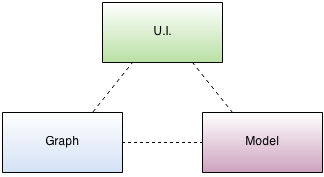
\includegraphics[width=0.4\textwidth]{images/initial_architecture.png}
    \caption{Architectural layout at the start of MPP2}
    \label{fig:initial_architecture}
\end{figure}

\begin{figure}[h!]
    \centering
    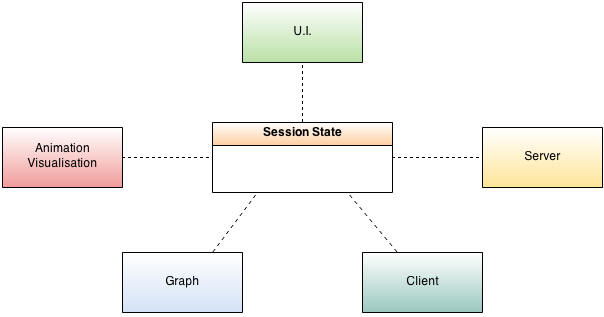
\includegraphics[width=0.6\textwidth]{images/final_architecture.png}
    \caption{Architectural layout at the end of MPP2}
    \label{fig:final_architecture}
\end{figure}

\begin{figure}[h!]
    \centering
    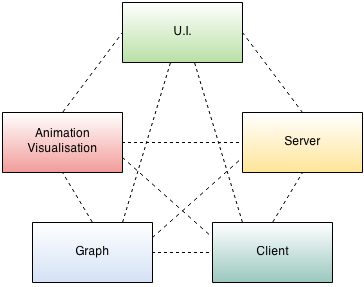
\includegraphics[width=0.4\textwidth]{images/initial_architecture_future.png}
    \caption{Architectural layout at the end of MPP2 if initial architecture was continued.}
    \label{fig:initial_architecture_future}
\end{figure}


\begin{figure}[h!]
    \centering
    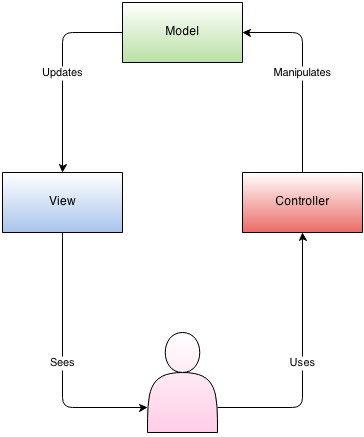
\includegraphics[width=0.4\textwidth]{images/mvc.png}
    \caption{Basic \ac{MVC} architecture}
    \label{fig:mvc}
\end{figure}

\afterpage{%
    \clearpage% Flush earlier floats (otherwise order might not be correct)
    \begin{landscape}
        \begin{figure}
            \centering
            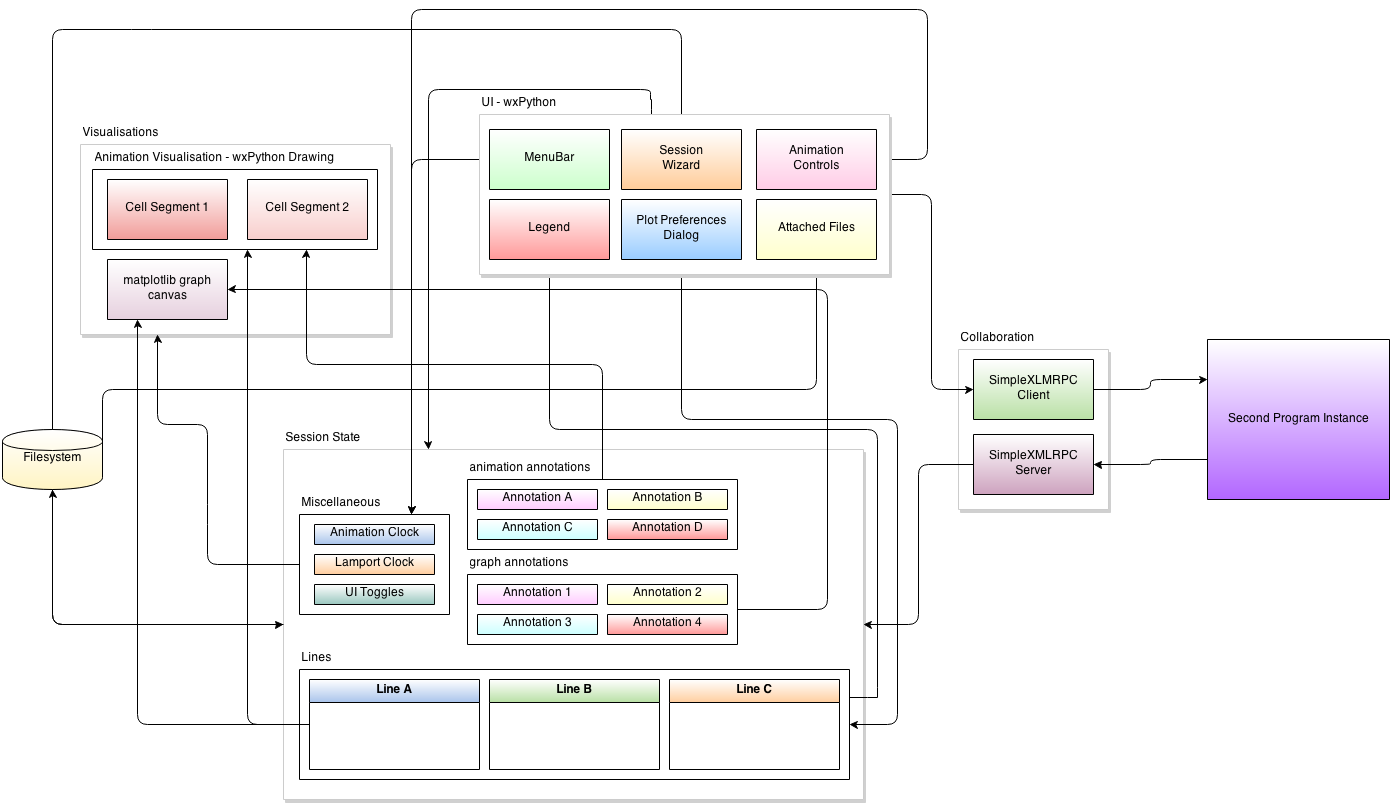
\includegraphics[height=0.9\textheight]{images/detailed_architecture.png}
            \caption{Detailed breakdown of program components and how they interact}
            \label{fig:detailed_architecture}
        \end{figure}
    \end{landscape}
}



\section{Animation}
\label{sec:animation}

Animation was a key goal of the project.  The core aim of the project was to help biologists who are not comfortable with traditional time-series graphs.  The goal was to provide them with visualisations closer to what they see in their domain.  This has been accomplished by displaying spatial data in the shape of a cross-section of a cell.

The animation is ideally used to display species moving through a cell.  This collapses what would be multiple different lines in a graph, that give no indication of their real position in the cell, into a single image.  This can be seen in Figure~\ref{fig:asrc_work}.

\begin{figure}[h!]
    \centering
    \begin{subfigure}[b]{0.4\textwidth}
        \centering
        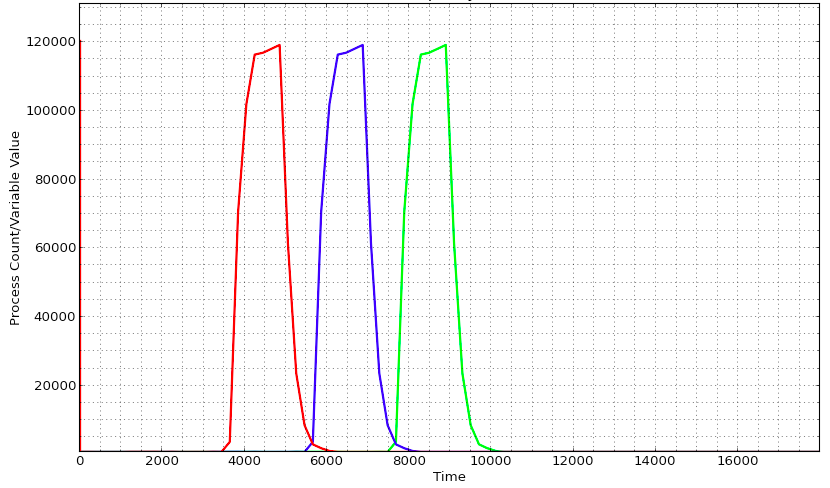
\includegraphics[width=0.8\textwidth]{images/asrc_graph_intro.png}
        \caption{Time series representation}
        \label{fig:asrc_graph_work}
    \end{subfigure}
    \begin{subfigure}[b]{0.4\textwidth}
        \centering
        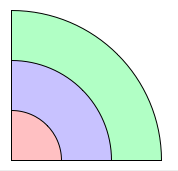
\includegraphics[width=0.5\textwidth]{images/asrc_cell_intro.png}
        \caption{Spatial representation}
        \label{fig:asrc_cell_work}
    \end{subfigure}
    \caption{One species at three locations in the cell represented traditionally on a time series graph and also spatially in a cell}
    \label{fig:asrc_work}
\end{figure}

Animation is just a sequence of static images which, when viewed frame by frame at a sufficient rate, will appear to be a dynamic image.  There are two basic ways that animation can be implemented: rendering the entire animation before it is required, or generating a static image as a function of time and every frame calculating what the image should be and displaying that to the user.  Both approaches have their advantages and disadvantages.  The most appropriate depends on the situation.  These options and how they would affect this project are reviewed below.

Rendering the animation before it is needed is not the correct way to do animation in this circumstance.  One of the purposes of this tool is to allow for interactivity and customisation.  This would potentially lead to the animation having to be rendered multiple times.  The animation that was planned to be included in this tool is also not complex enough to warrant pre-rendering.  Pre-rendering would be more suitable for more realistic animations.  One would be doing this after the insight has been learned from the experimental data.  The purpose of the animation here is to help the user to find this insight.  For these reasons treating animation as generating static images as a function of time was chosen.

We had to decide how the animation would be displayed.  wxPython and matplotlib are both used for visual display in this project.  It made sense to implement animation using one of them.  The capabilities of implementing animation was investigated for choices before the decision was made.  The findings are below.

wxPython does not have built-in animation support but it does, however, have built-in drawing support through the paint device context.  This allows for arbitrary drawing on \ac{UI} panels.  wxPython also provides some drawing primitives.  Various primitives can be handled such as squares, circles, triangles and text.  There is also support for drawing arcs.  These primitives can be combined to form regions allowing more complex shapes to be drawn.  During the planning phase (MPP) it was decided to draw cell cross-sections.  These cell cross-sections were going to be arcs.  wxPython providing support for arcs was perfect for this.  This approach would be most suitable for generating images as a function of time.

matplotlib does have support for animation with the matplotlib.animation library.  This implements animation as a function of time.  To display animations matplotlib requires: a function that generates the data to be plotted (which will change depending on the time value) and the interval of time between frames.  matplotlib also has support for shapes.  Each cell cross-section could then be treated as a separate matplotlib animation.  matplotlib would also require a canvas to draw on.  The appearance of this canvas would have had to be customised to make the animation look less like a graph, for example removing ticker lines from the axis.  This would be a lot of scaffold code to implement animation.

wxPython and matplotlib's animation capabilities are quite similar, both have primitives for drawing the necessary shapes and both are implemented as drawing static images as a function of time.  Given that the capabilities of each were similar wxPython was chosen for animation to avoid the scaffolding code that matplotlib would have required.  This enabled animation to be developed faster.

The animation visualisation will usually be one or more cell cross-sections.  Each cross-section is split into compartments. These compartments are parsed from the model file.  In the model file compartments are stored hierarchically.  The structure of the cell in the model can be inferred from this hierarchy.  Each compartment in the model relates to one segment in the cell cross-section.  wxPython's built-in arc drawing was used to draw the cross-sections.  The cross-section has to be drawn from the edge of the structure into the centre.  Each arc is drawn on top of what is already there.  If the larger outer arcs were drawn last then they would cover the inner arcs.  The division of the cell cross-section is such that every visible segment has the same width.  An example cell cross-section can be seen in Figure~\ref{fig:cell_segment}

\begin{figure}[h!]
    \centering
    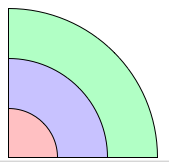
\includegraphics[width=0.3\textwidth]{images/cell_segment.png}
    \caption{A cell cross-section formed of three segments.}
    \label{fig:cell_segment}
\end{figure}

Over the course of the animation the colour of the segment changes to reflect the colour in the intensity plot version of the line.  This allows the researcher to compare the two visualisations and will hopefully help build their confidence understanding the graph plot.

Animation takes advantage of the data-centric model.  When the play button is pressed a thread is created whose job it is to increment the animation clock and refresh all the \ac{UI} elements.  When refreshed the \ac{UI} elements pick up on the change of clock and update what they display appropriately.

The first step towards animation was calculating at what points the line changes colour.  This is done during the interpolation phase that was implemented in the first stage of development.  To do the interpolation the original plot is split into multiple separate plots with the results padded with null values to allow matplotlib to plot them as one.  This is detailed further in the report for MInf Project Phase 1.  The number of these null values is counted and that gives the time at which the colour should change.  This is stored as an array of time, colour tuples.  Each line also has an internal counter to say how many elements into this array the line is.  When the animation clock is updated and the refresh triggered, each cell segment finds the appropriate colour change point in the line by going through the array and comparing each time to the animation clock until the time is found and updates the segment colour.  This position is then used as the new starting point on the next refresh.  This removes the need to look through past entries unnecessarily.

\tdi{put some more figures in, I think an annotated cell cross-section could b good}

The user can control the animation clock through the time slider.  Moving the time slider updates the animation clock to be the value of the time slider and triggers a refresh of all the cell segments. This ensures that the user is seeing up to date information.   As described above, each line has a list of times at which it changes colour.  These are sorted according to time.  During `normal' animation the previous position in the array is tracked so that the whole array is not searched every time unnecessarily.  When the time slider is used this previous position might become a future position.  To solve this the previous position is set back to the start of the array.  On the next refresh the array will be searched from the start for the appropriate time and colour.

A nice \ac{UX} feature that has been added is a line on the main graph that indicates the current time in the animation. This can be seen in Figure~\ref{fig:animation_clock}.  When the animation is running the line moves along the graph.  This again helps the user build a correspondence between the two visualisation types and may help with their understanding of what is being displayed on the graph.

\begin{figure}[h!]
    \centering
    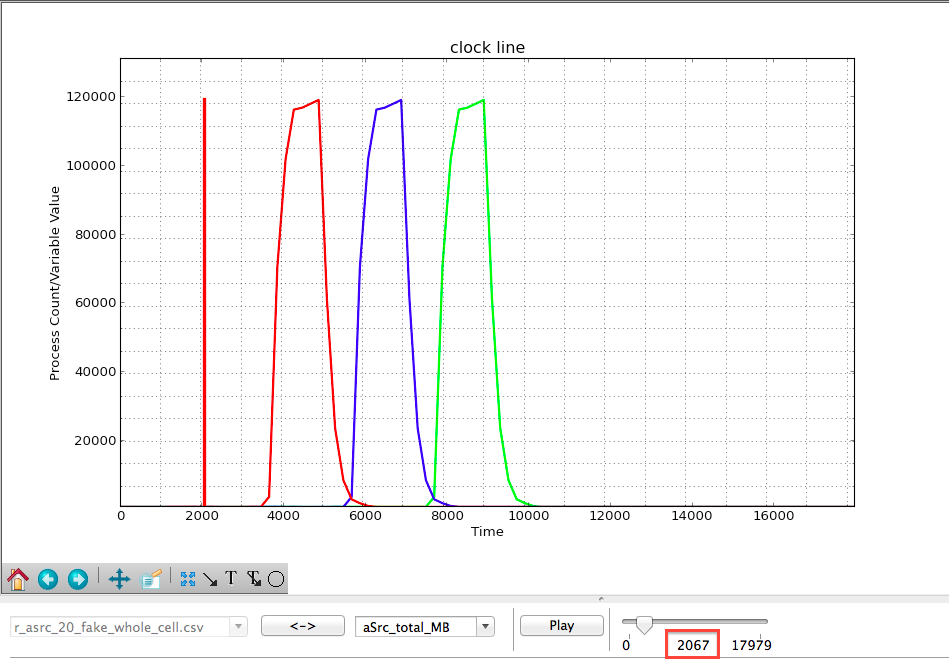
\includegraphics[width=0.8\textwidth]{images/animation_clock_line.png}
    \caption{Vertical line that is drawn on the graph to indicate current animation clock time.}
    \label{fig:animation_clock}
\end{figure}

The user is also given control over what is displayed.  The cell cross-sections can be drawn in a file-focussed manner or a species-focussed manner.  In the file-focussed manner a cell cross-section is drawn for every species in that file.  The user can switch between all results files that have been added to the session.  In the species-focussed manner a cell cross section is drawn for every file that contains that species.  The user can select between all species found across all the results files.  These are illustrated in Figure~\ref{fig:cell_segments}

Figure~\ref{fig:cell_segments} shows example cell cross-sections.  Figures~\ref{fig:cell_seg_file_fake}~\&~\ref{fig:cell_seg_file_model} show the cell cross-sections being drawn in the file-focussed manner.  Both files contained results relating to the the species ``aSrc\_total\_MB". In Figure~\ref{fig:cell_seg_file_fake} this species was present at all locations in the cell.  In Figure~\ref{fig:cell_seg_file_model} the species is missing from the middle location in the cell.  The middle segment has been left white to indicate this.  Figure~\ref{fig:cell_seg_species} shows the cell segments drawn in a species-focussed manner.  One cell cross-section has been drawn for each file which contains the species ``aSrc\_total\_MB''.  We can see that in one of the files the species wasn't present at all locations.

\begin{figure}[h!]
    \centering
    \begin{subfigure}[b]{0.9\textwidth}
        \centering
        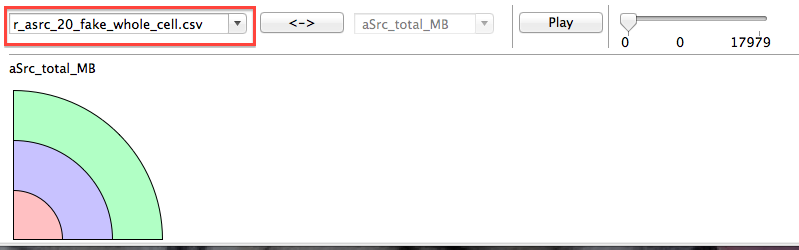
\includegraphics[width=\textwidth]{images/by_file_fake.png}
        \caption{Cell segments drawn by species from file r\_arsrc\_20\_fake\_whole\_cell.csv}
        \label{fig:cell_seg_file_fake}
    \end{subfigure}

    \begin{subfigure}[b]{0.9\textwidth}
        \centering
        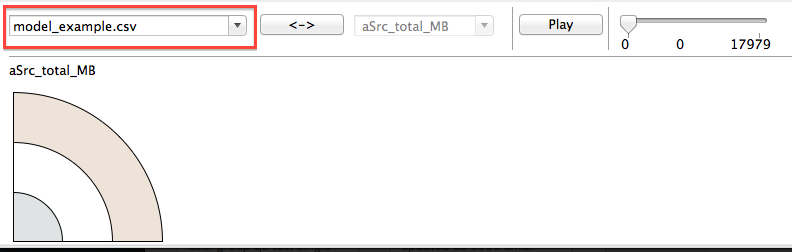
\includegraphics[width=\textwidth]{images/by_file_model.png}
        \caption{Cell segments drawn by species from file model\_example.csv}
        \label{fig:cell_seg_file_model}
    \end{subfigure}

    \begin{subfigure}[b]{0.9\textwidth}
        \centering
        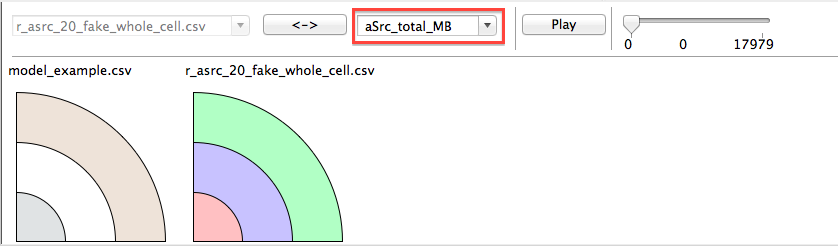
\includegraphics[width=\textwidth]{images/by_species_asrc.png}
        \caption{Cell segments drawn by file from species aSrc\_total\_MB}
        \label{fig:cell_seg_species}
    \end{subfigure}
    \caption{Example cell segment animations}
    \label{fig:cell_segments}
\end{figure}

It had been hoped to allow the user to save the animation.  This could have been implemented by either allowing the user to save individual frames, or allowing the user to save an animated gif of the whole animation.  Saving to a gif was chosen as it was felt to be more useful, to a user, to be able to export the entire animation rather than a single frame of it.  Allowing the user to save a single frame would be added in at a future date.  To generate the gif we need to save all frames.  As these frames are generated as needed, not pre-rendered it was required to run through the whole animation to save each frame.  This meant that saving all the frames took as long as the animation took to run.  At this stage in the save animation process, hundreds of static images have been saved.  A shell script is then required to convert the saved frames into a gif.  Given that this was a very slow and user unfriendly approach the decision was made to remove the ability to save animation from the project.  It would, hopefully, be implemented if future work was to be performed.

\section{Annotation}

Annotation was an important feature to add.  It is one of Grinstein's features that data visualisation software should have~\cite{gg_vizbi}.  This is because the purpose of a visualisation is to aid analysis.  If you have a print out of a visualisation you are able draw on it and highlight areas of interest.  Users need to be able to do this on digital versions of their visualisations.  As well as helping users analyse their data, being able to annotate also means that images for presentations can be prepared without having to save the visualisation and open it in an external program.  If you did this and then wanted to change the visualisation you would have to re-annotate it.  This is frustrating for a user and wastes their time.  Being able to do the annotation from within the visualisation solves this problem as the raw data and the annotation data are together.  Another benefit of being able to annotate is having another way of attaching additional information to the visualisation when sending it to a colleague. Having this information on the visualisation saves the colleague from flicking back and forth from an email or other supporting documentation.

Implementing annotation of the visualisations on offer in this tool had to be done in two parts.  This is because there are two parts to the visualisation:  the graph and the cell level animation.  One is a static visualisation and one is a dynamic visualisation.  Each of these required a different approach.  These are detailed below.

\subsection{Annotation of the Graph}
\label{sec:annotation_graph}

Annotations of a static image are extra elements that are added by the user.  We needed to decide what extra elements we are going to allow the user to add.  We also needed to decide how to render the annotations.

For this project there are two options for drawing the annotations on the graph: with matplotlib, or with wxPython.  matplotlib has support for annotations.  In matplotlib annotations have two forms. The first form uses the annotate() and text() functions which, respectively, add an arrow with optional text to the graph and add text without an arrow to the graph.  matplotlib's second form uses its artists and patches library.  With these libraries arbitrary shapes and different forms of arrow can be added.  The other option was drawing the annotations with wxPython.  As in Section~\ref{sec:animation} we can use device contexts to draw primitives on \ac{UI} elements with wxPython.  The primitives offered by the device context do not include arrows which are a key annotation type.  In Section~\ref{sec:animation} wxPython was chosen over matplotlib partially because using matplotlib would have involved more scaffolding code.  For annotating on the graph this scaffolding code is already there from the creation of the graph.  As wxPython had a better range of primitives and needed less supporting code it was chosen to implement annotation on the graph using matplotlib's support.

\tdi{Make it clearer that a decision is being made}

matplotlib's support for elements on the graph is quite thorough.  Text and arrows are obvious choices as they allow the user to indicate and explain areas of interest.  matplotlib then allows for more arbitrary drawing.  So as to not overload the user with annotation choices it was decided to limit the number of annotation elements that they could use.  In addition to the text and arrows the user can also add circles as an annotation.

Users of the new tool are provided with four annotation types: arrow, text, arrow with text and circles.  Buttons for each of these annotation types have been placed on the matplotlib toolbar.  This can be seen in Figure~\ref{fig:annotation_demo}.  These four annotation types come from different libraries within matplotlib.  An annotation class was defined to attempt to abstract their differences.  This would also make it easier were more annotation elements to be added in the future.

\begin{figure}[h!]
    \centering
    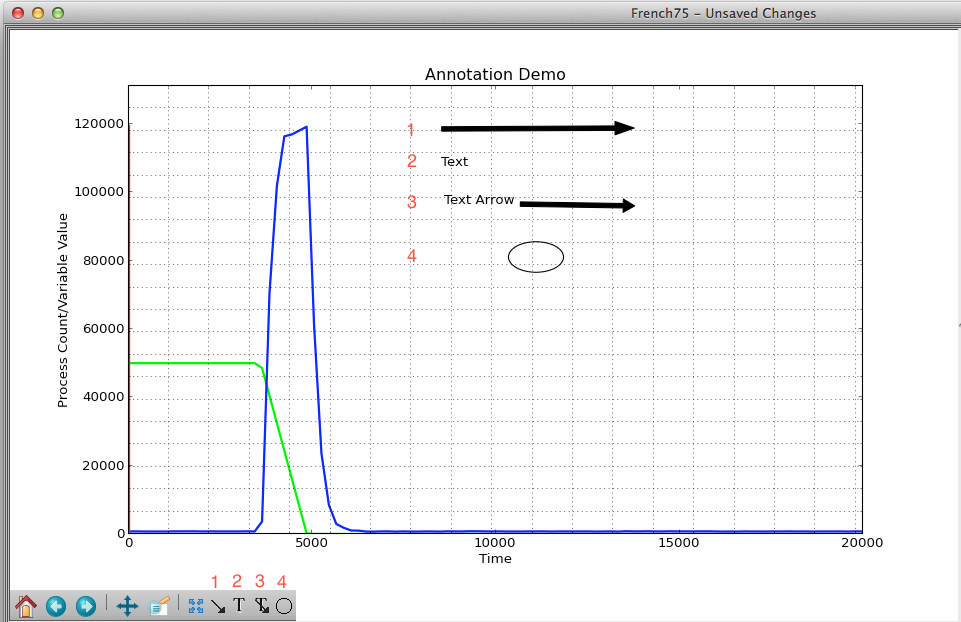
\includegraphics[width=\textwidth]{images/annotation_demo.png}
    \caption{Example of each of the four graph annotation types and the toolbar buttons that correspond to them.}
    \label{fig:annotation_demo}
\end{figure}

There were problems in making the annotation creation process user friendly.  For all of the annotations the user needs to first press the appropriate button on the toolbar.  The next actions depend on the annotation type.  Text and circle annotations were intuitive as all they require is one click.  The user clicks where they want the annotation to be placed and it will be drawn on the graph there.  However the arrow annotation types required two clicks.  The first click marks the start point (the tail of the arrow) and the second click is the finish point (the head of the arrow).  This was not obvious. User evaluations revealed that the users did not know that it required two clicks and didn't know whether the arrows would be drawn head to tail or tail to head.  The technique for placing arrows was subsequently changed so that the first click still fixed the position of the tail of the arrow. However the behaviour after the first click changed, so now a temporary annotation is continuously redrawn that has the head of the arrow wherever the cursor is.  This allows the user to see the arrow they are drawing.  To indicate to the user that they need to click on the graph the cursor is changed after pressing one of the annotation buttons on the toolbar.  The use of different cursors is a common technique to help guide users to perform actions.

It was important that annotations could be edited or deleted.  Recoverability from error is an import \ac{HCI} guideline~\cite{shgold}\cite{normsev}\cite{neilten}.  The annotations can not just be clicked as they are not a \ac{UI} widget like a button.  The solution to this was to have an array of annotations.  When a user right clicks on the graph it searches through all annotations and selects the annotation that was closest to the click (if that distance was below a certain threshold).  The selected annotation is then highlighted red, and a context menu appears to give feedback to the user that they have successfully selected an annotation.  This can be seen in Figure~\ref{fig:annotation_selection}.  The context menu then gives the user the option to edit or delete an annotation.  Editing an annotation only allows for editing text.  For changing position, the annotation has to be deleted and redrawn.

\tdi{How does the user know there is a context menu?  In evaluations pretty much everyone has failed}

\begin{figure}[h!]
    \centering
    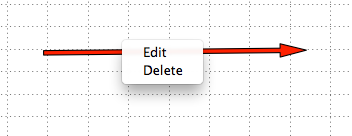
\includegraphics[width=0.6\textwidth]{images/annotation_selection.png}
    \caption{Context menu on selection of graph annotation.}
    \label{fig:annotation_selection}
\end{figure}

To calculate the distance from the location of the mouse click to the annotation two problems had to be solved.  The first was how to calculate the distance from a point to a line (This is only for the arrow annotations.  The text and circle annotations use standard point to point Euclidean distance).  An equation for this can be seen in Figure~\ref{fig:point_to_line_eq}.  Equation~\ref{eq:line} is the equation for a line in two dimensions.  This represents the annotation.  The equation can be calculated from the start and end points of the annotation. Equation~\ref{eq:point} is the position of the mouse click.  Equation~\ref{eq:distance} shows the equation for calculating the distance from the point to the line.  The second problem that had to be overcome was the difference in scale.  In effect we have two coordinate systems.  The results coordinate system and the visual coordinate system.  The difference is illustrated in Figure~\ref{fig:distance_scale}.  The annotations in Figure~\ref{fig:distance_scale_a} are further away from each other in the results coordinate system than the annotations in Figure~\ref{fig:distance_scale_b}. However they are closer in the visual coordinate system.  When selecting an annotation the user is using the visual coordinate system but the distance is calculated using the result coordinate system.  This could lead to the wrong annotation being selected.  The solution to this was to transform one coordinate system into the other.  When calculating the distance from the point to the line, the values are scaled by the size of the graph.

\begin{figure}[h!]
    \centering

    \begin{subfigure}[b]{\textwidth}
        \centering
        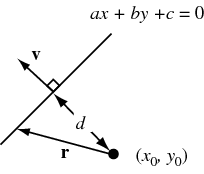
\includegraphics[width=0.3\textwidth]{images/point_to_line.png}
        \caption{Diagram of the point to line distance problem}
        \label{fig:point_to_line_diagram}
    \end{subfigure}

    \begin{subfigure}[b]{\textwidth}
        \begin{subequations}
            \begin{align}
            & y = -\frac{a}{b}x - \frac{c}{b} \label{eq:line}\\
            & (x_{0}, y_{0}) \label{eq:point} \\
            & d = \frac{\mid ax_{0} + by_{0} + c \mid}{\sqrt{a^{2} + b^{2}}} \label{eq:distance}
            \end{align}
        \end{subequations}
        \caption{Equations for calculating the distance from a point to a line.}
        \label{fig:point_to_line_equations}
    \end{subfigure}
    \caption{Equations and diagram for dalculating the distance from a point to a line (taken from WolframMathWorld~\cite{point_to_line})}
    \label{fig:point_to_line_eq}
\end{figure}

\begin{figure}[h!]
    \centering
    \begin{subfigure}[b]{0.6\textwidth}
        \centering
        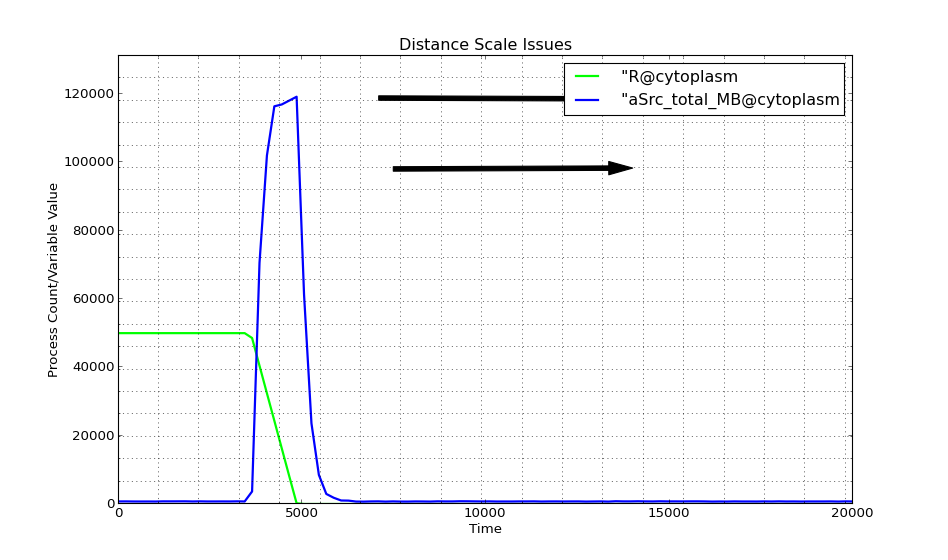
\includegraphics[width=\textwidth]{images/distance_scale_a.png}
        \caption{Annotations with distance of approximately 20000}
        \label{fig:distance_scale_a}
    \end{subfigure}

    \begin{subfigure}[b]{0.6\textwidth}
        \centering
        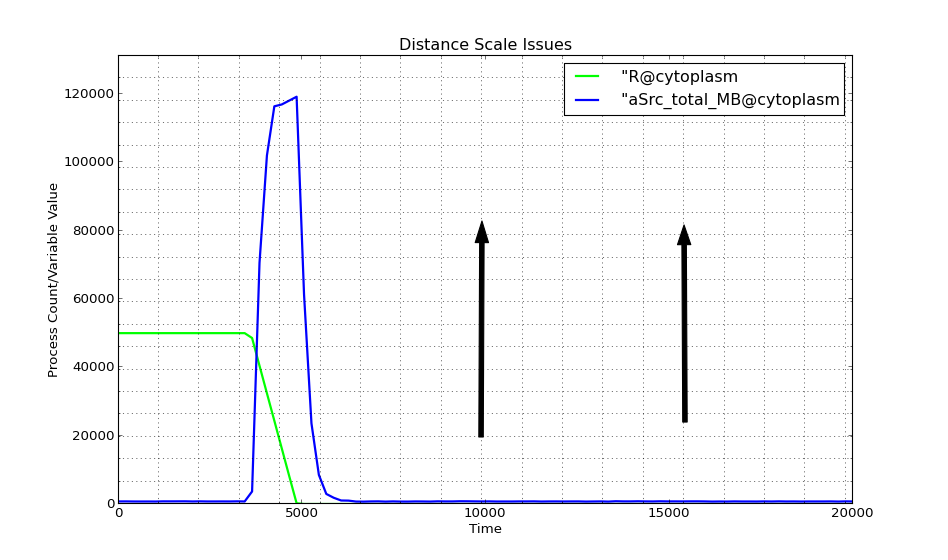
\includegraphics[width=\textwidth]{images/distance_scale_b.png}
        \caption{Annotations with distance of approximately 5000}
        \label{fig:distance_scale_b}
    \end{subfigure}
    \caption{Two sets of annotations illustrating the problems when calculating the distance to an annotation}
    \label{fig:distance_scale}
\end{figure}

A similar issue to the difference in scale when calculating the distance from the mouse to annotation was encountered when switching the graph to display the normalised data (described in Section~\ref{sec:normalised}).  When normalised the graph in the y axis only goes between 0 and 1.  The coordinates of the annotation are likely to be very much outside this range and the annotation would not appear on the graph.  The solution, if the graph was normalised, was to normalise the positions of the annotations in the y axis when drawing them.  A side effect of this technique is that after the lines are rescaled.  The annotations could be left pointing to nothing.  This is unavoidable as the annotation has no concept of what it is pointing at.  It may be pointing to the intersection of many lines; in this case it would be impossible to keep the annotation pointing at what it was originally pointing at after rescaling the axis.  During user evaluations, when the annotation was not visible during data normalisation, the user was very confused as to why their annotation had disappeared.  It was therefore decided that having the annotation be visible but most likely incorrect is more user friendly than just not displaying the annotations.  Not displaying the annotations looks like a serious error.

\begin{figure}[h!]
    \centering
    \begin{subfigure}[b]{0.6\textwidth}
        \centering
        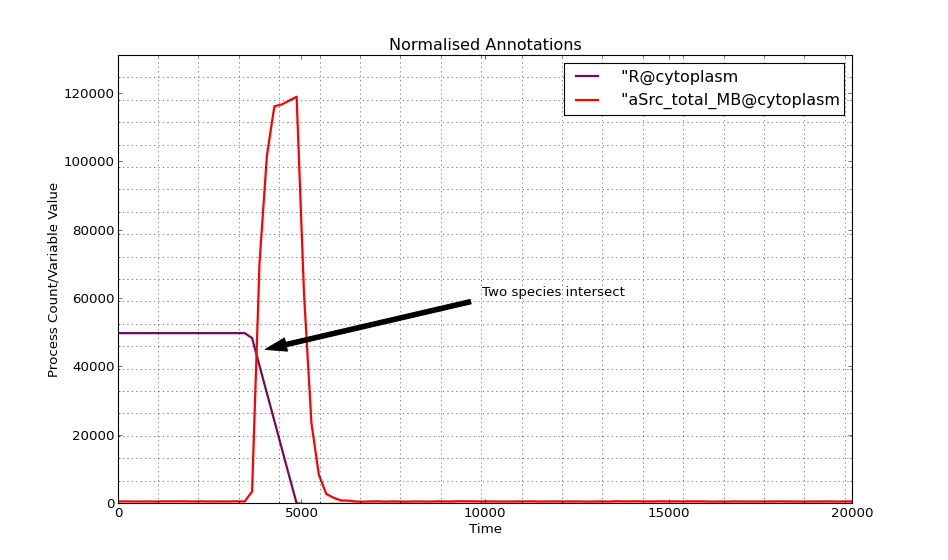
\includegraphics[width=\textwidth]{images/unnormalised_annotation.png}
        \caption{Annotation pointing at the correct intersection of species}
        \label{fig:annotation_instersection_a}
    \end{subfigure}

    \begin{subfigure}[b]{0.6\textwidth}
        \centering
        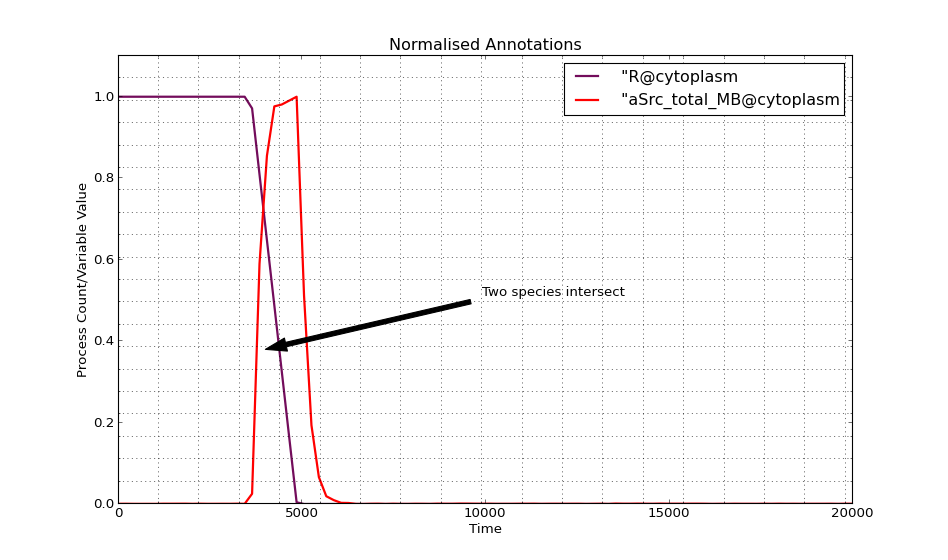
\includegraphics[width=\textwidth]{images/normalised_annotation.png}
        \caption{Annotation pointing at nothing after data normalisation}
        \label{fig:annotation_intersection_b}
    \end{subfigure}
    \caption{Graphs illustrating what happens to annotations whilst data is normalised}
    \label{fig:annotation_intersection}
\end{figure}

\subsection{Annotation of the Animation}
\label{sec:anime_annotation}

After completing annotation of the graph it was important to expand this to the animation panel, as this is the other visualisation option available to a user.  Annotating animations posed more of a challenge than annotation of the graph and there were a number of issues to overcome.

\begin{enumerate}
\item How to implement the annotations?  For the graph matplotlib has built-in annotation support.  wxPython does have drawing support but not built-in annotation support.  Annotating on the animation will need manual handling of the drawing on top of the animation visualisation.  Manual drawing means that the automatic layout functionality that wxPython provides cannot be used.
\item When to display the annotations?  When an annotation is drawn on the graph it is displayed at all times.  The appearance of the graph does not change over time.  However the appearance of the animation visualisation does change over time.  The problem faced when annotating is whether to have annotations available at only specific times in the animation, or to have them there the whole time; and if they are going to appear and disappear, how can it be done without being distracting?
\item How to give the user control over the annotations? When a user wants to edit or delete an annotation on the graph it is always there.  However on the animation panel if the annotation is temporal, then it is not always visible for the user to edit or delete and it would be frustrating for a user to constantly have to search through the animation to look for annotations to change them.
\end{enumerate}

A platform where users are able to annotate an `animation' is YouTube~\cite{youtube}.  YouTube's annotation interface can be seen in Figure~\ref{fig:youtube}.  YouTube's approach is to allow the user to set what period of time an annotation is visible for.  There is also a management panel where the user can see all of the annotations and edit or delete them.  This approach solved issues two and three and was adapted for this tool.

\begin{figure}[h!]
    \centering
    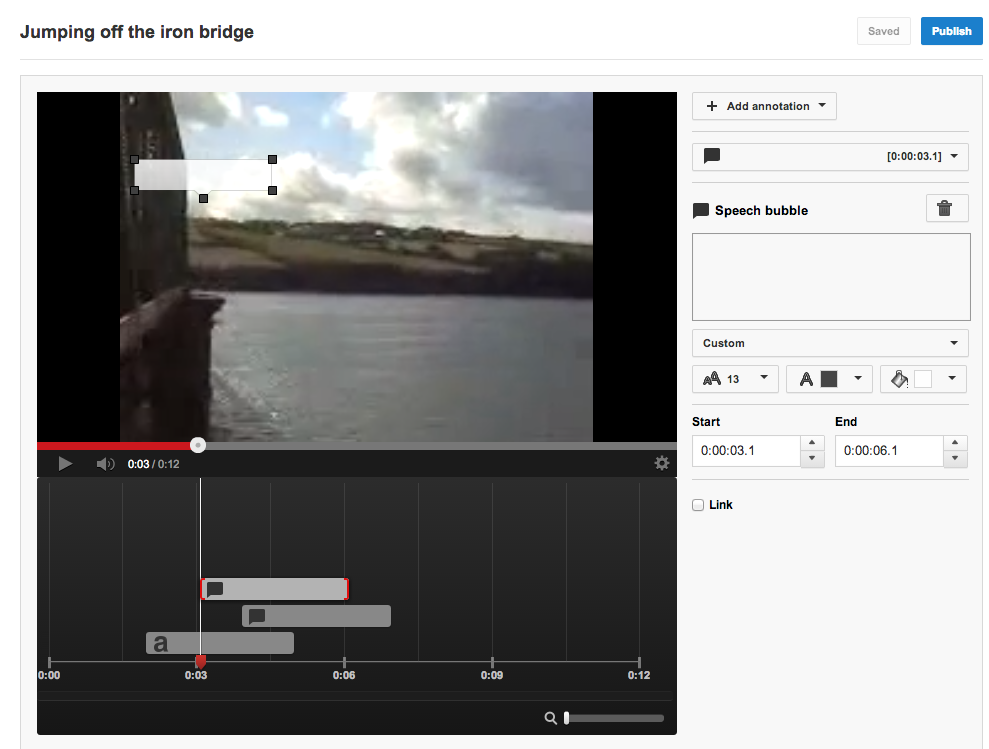
\includegraphics[width=0.7\textwidth]{images/youtube.png}
    \caption{YouTube video annotation interface}
    \label{fig:youtube}
\end{figure}

On the right hand side of the tool there is a panel which lists all annotations that have currently been added to the tool, this can be seen in Figure~\ref{fig:annotation_list}.  This provides the user with the persistent view of what has been added.  When the user creates an annotation they are shown a dialogue that allows them to enter the annotation text and to choose a duration. This can be seen in Figure~\ref{fig:annotation_dialog}. The duration indicates to the user that the annotation will only be visible at certain times.  The start and end times are given in model time.  The duration displayed to the user is given as the real time that the annotation will be visible for.

\begin{figure}[h!]
    \centering
    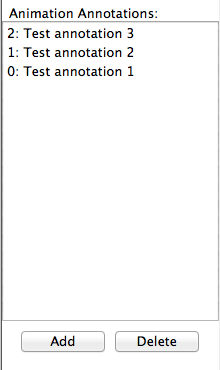
\includegraphics[height=0.4\textheight]{images/annotation_list.png}
    \caption{Animation annotation list}
    \label{fig:annotation_list}
\end{figure}

\begin{figure}[h!]
    \centering
    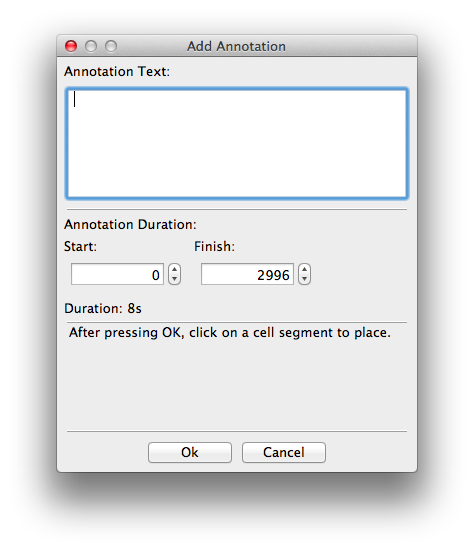
\includegraphics[width=0.7\textwidth]{images/annotation_dialog.png}
    \caption{Animation annotation dialogue}
    \label{fig:annotation_dialog}
\end{figure}

The first problem -- how to display the annotations -- has also been solved.  Drawing in wxPython takes place on panels.  Each cell cross-section is placed on its own panel.  This drastically limits the available space.  The panels are not wide enough to have the annotation text drawn on.  The solution was to assign each annotation a number and that number is what is used to annotate the cell.  The number is then displayed in the annotation list box allowing the user to read the appropriate annotation.  This can be seen in Figure~\ref{fig:annotation_whole}

\begin{figure}[h!]
    \centering
    \begin{subfigure}[b]{0.4\textwidth}
        \centering
        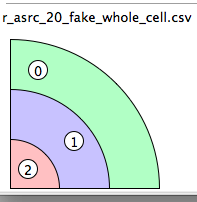
\includegraphics[width=0.9\textwidth]{images/annotation_whole_b.png}
        \caption{Annotated cell cross-section}
        \label{fig:annotation_whole_cell}
    \end{subfigure}
    \begin{subfigure}[b]{0.4\textwidth}
        \centering
        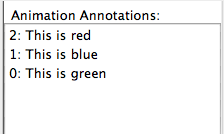
\includegraphics[width=0.9\textwidth]{images/annotation_whole_a.png}
        \caption{Corresponding annotation List}
        \label{fig:annotation_whole_list}
    \end{subfigure}
    \caption{Animation annotations}
    \label{fig:annotation_whole}
\end{figure}

\section{Search}
\label{sec:search}

Being able to use a time series graph as a query against a database of time series data was one of the new goals added to the project.  It was felt it would be of great use to the biologists as it would allow for discoverability within the tool.  It had been identified as a potential goal whilst researching data mining in time series data.  It was added as a definite project goal after the user group backed it as a feature they would very much like to have.  It is also a feature in the tool that incorporates cross-domain knowledge in an area of active research.

\tdi{Emphasize the challengingness}

Some problems needed to be overcome before using plots as a query could become useful:
\begin{itemize}
\item How to cope with different scales?
\item How to cope with events happening at different times?
\item How to represent the plot to allow for efficient search?
\item How to determine similarity between two graphs?
\end{itemize}

Early techniques used simple similarity measures such as Euclidean distance, but these gave poor results~\cite{chotirat}.  The reason for the poor results is that Euclidean distance does not take into account scale or time.  Figure~\ref{fig:similar} illustrates a case where Euclidean distance would give a poor similarity measure.  The two lines are identical, but the green line has been shifted in time.  Euclidean distance will not recognise that they are similar.  The same problem would happen if one line had been shifted in the y-axis above the other.

\begin{figure}[h!]
    \centering
    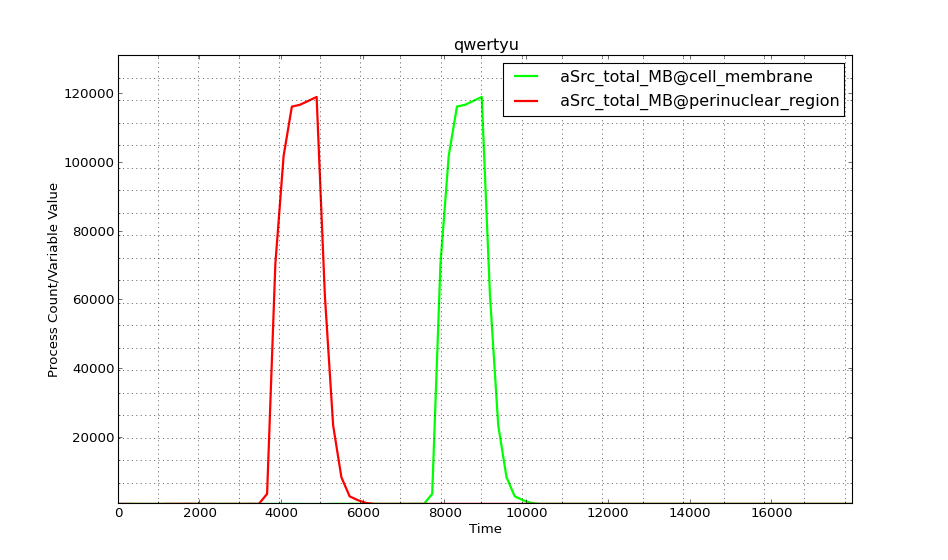
\includegraphics[width=0.7\textwidth]{images/similar_plots.png}
    \caption{Identical plots shifted in time}
    \label{fig:similar}
\end{figure}

It is important to define what it means for two lines to be similar.  It is obvious that in a case such as Figure~\ref{fig:similar} that the two lines are similar.  Both lines are the same shape and they are exhibiting the same behaviour.  When determining similarity of plots we should take a time invariant approach.  Perhaps less obvious is the case where we have offset in the Y-Axis as shown in Figure~\ref{fig:similar_y}.  Figure~\ref{fig:similar_1} shows two identical lines where one line had an additional 100000 population level.  Figure~\ref{fig:similar_2} shows two lines where one line is double the other line.  Figure~\ref{fig:similar_1} is effectively the same case as Figure~\ref{fig:similar}.  Figure~\ref{fig:similar_2} is different, but it is clear looking at the graph that they are exhibiting the same behaviour. When determining the similarity of plots we should take a scale invariant approach~\cite{esling}.

\begin{figure}[h!]
    \centering
    \begin{subfigure}[b]{0.6\textwidth}
        \centering
        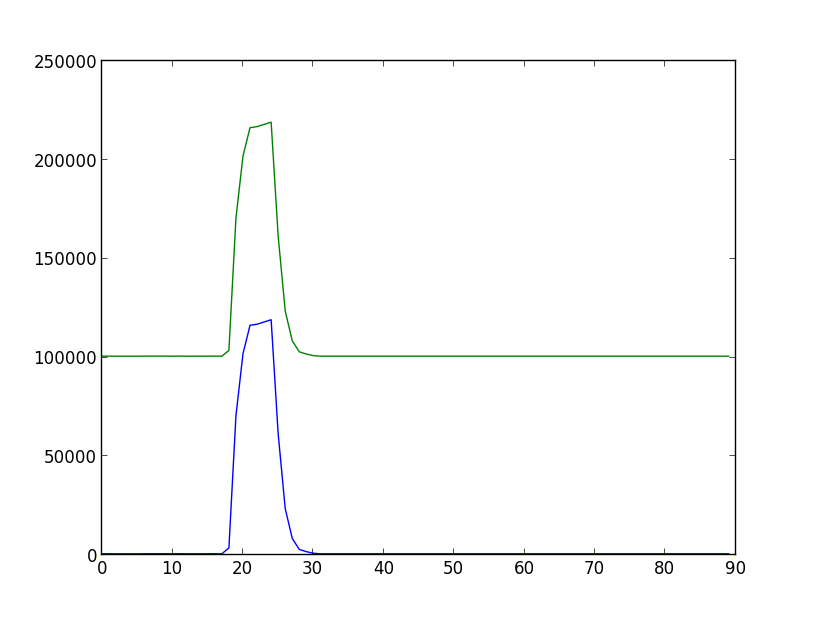
\includegraphics[width=0.7\textwidth]{images/similar_plots_2.png}
        \caption{Identical plots shifted in population level}
        \label{fig:similar_1}
    \end{subfigure}

    \begin{subfigure}[b]{0.6\textwidth}
        \centering
        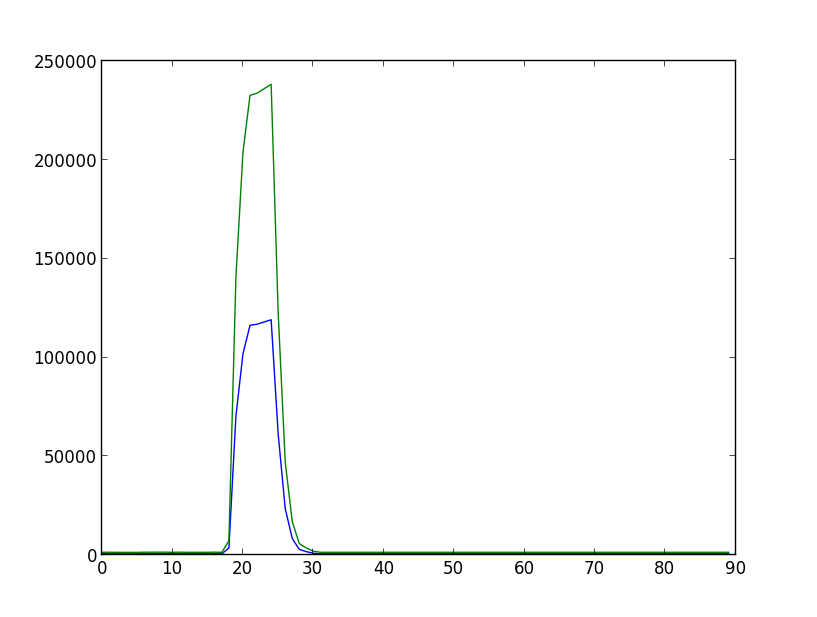
\includegraphics[width=0.7\textwidth]{images/similar_plots_3.png}
        \caption{Identical plots scaled in population level}
        \label{fig:similar_2}
    \end{subfigure}
    \caption{Graphs illustrating different ways lines can be offset in the y-axis}
    \label{fig:similar_y}
\end{figure}

Approaches that have been researched to determine similarity between time series data have included shape based approaches and dynamic programming techniques.  Not all of these approaches have included dimensionality reduction.  The dimensionality reduction transforms the input data into a vector space with fewer dimensions.  Similar values in the data space will, in theory, be transformed to the same value in the vector space.  The need for dimensionality reduction is explained later in this section.  After researching alternatives an approach was adapted from the work of Lin \& Li~\cite{structural_similarity}.

Lin \& Li's approach uses normalised sub sequence data to reduce the dimensionality of the dataset.  The reduced data can then be used to efficiently find the most similar plots in the database.  The input data is converted into sub lists to ensure that all features will have been captured.  These lists are then normalised and have their dimensionality reduced.  This is where Lin \& Li's work left the topic.  Work from the field of information retrieval was then applied to provide the similarity ranking. This approach is explained in further detail below.

The first step was to take the input data and return all the sub lists of this data.  To do this a sliding window was used.  The size of the sliding window will determine the feature size in the reduced vector.  Lin \& Li use a size of eight for the sliding window.  The same value was chosen in this implementation.  If we have input data $[1,2,3,4,5]$ and windows size $n = 3$ (for illustrative purposes only) then we get the sub lists as $[[1,2,3]$, $[2,3,4]$, $[3,4,5]]$.

The second step is to normalise each sub list.  Each sub list is normalised to be zero mean and unit variance.  This places each sub list onto the same scale.  This removes the effect of the offsets seen in Figure~\ref{fig:similar_y}.  To normalise to zero mean and unit variance we need the mean ($\mu$) and the standard deviation ($\sigma$).  We then have:

$$
\left[\frac{x - \mu}{\sigma},\text{   } \forall x \in sublist\right]
$$

The third step is to reduce the dimensionality of the data.  Lin \& Li's approach also involves converting the data from a continuous representation into a discrete representation.  By normalizing the sub lists to be zero mean and unit variance we allow a Gaussian distribution to be fitted to the data.  This can be seen in Figure~\ref{fig:gaussian_plot}.  This approach does assume the Gaussian distribution is a suitable distribution.  Lin \& Li found it to be a suitable distribution but do note that other distributions could be investigated; this was outside the scope of this project.  For each data point we use the Gaussian function and map it to a letter.  This can be seen in Figure~\ref{fig:gaussian_plot} which shows a line formed of eight datapoints, our sublist, that have been normalised to be zero mean and unit variance.  Each datapoint has been mapped to one of the three sections of the distribution divided by the breakpoint and has been replaced with the letter that represents that section.  Breakpoints are used to divide the Gaussian distribution into sections with equal probability.  To split the distribution into three sections two breakpoints are needed. The values of these breakpoints can be found in statistical lookup tables.  If our breakpoints divide the distribution into three sections then each datapoint can be mapped to one of these three sections.  Lin \& Li divide their distribution into three sections and represent each section with a character.  They found three sections to be suitable, again alternative numbers of breakpoints could be used but this is outside the scope of the project.  This reduces the dimensionality of the dataset as multiple real values are mapped to a single letter.

After this stage each sublist has been transformed into an eight character long string.  The plot is represented as a list of strings.  These strings represent the features of the plot.

\begin{figure}[h!]
    \centering
    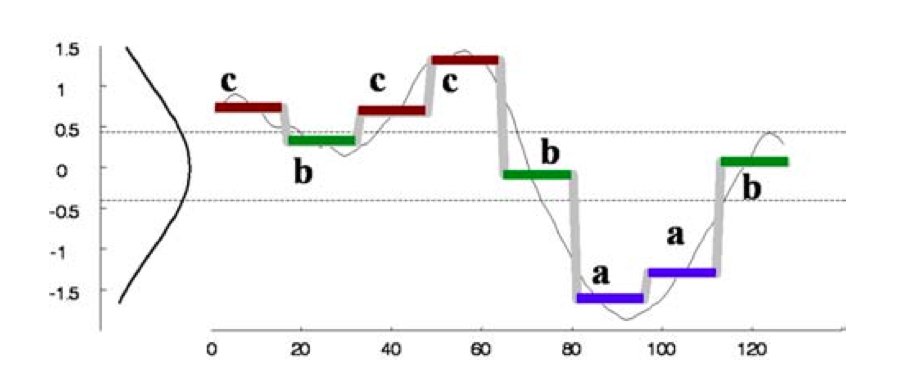
\includegraphics[width=\textwidth]{images/similiarty_normalise.png}
    \caption{Fitting a Gaussian distribution to time series data, taken from~\cite{structural_similarity}.}
    \label{fig:gaussian_plot}
\end{figure}

Lin \& Li now call for the removal of local duplicates within the list of features.  If we have runs of a certain feature then that should be reduced to a single instance of the feature.  For example, using a feature size of three, if we have the reduced representation $``AAA"$, $``AAA"$, $``BBA"$, $``BBB"$, $``BBB"$, $``AAA"$, $``AAA"$ it should be reduced to $``AAA"$, $``BBA"$, $``BBB"$, $``AAA"$ not $``AAA"$, $``BBA"$, $``BBB"$.  We are not removing all duplicates of the feature.  This reduces the number of entries in the representation and provides an efficiency benefit.  It will also remove the effect seen in Figure~\ref{fig:similar_2} where Euclidean distance would give a value indicating dissimilar if one line is a scaled version of the other.  This is because we have just removed long features with the same behaviour to be unit length features.

The plot is now represented as a list of strings without local duplicates.  Our strings all have a length of eight characters and the strings are composed from a three letter alphabet.  This gives us a vocabulary of $3^8$ possible features.  The index of the plot is a $3^8$ element vector where each entry in the vector contains the count of the feature in the line.  This is a very wasteful representation as most of the entries in the vector will be zero.  We can replace this with a sparse representation where we store only the features that make up the line and their count.

This representation of the plot also solves the problem of features being temporally located in the graph.  In the plot index there is no ordering of the features, in effect all the features happened at the same time.  This is a common representation in information retrieval and is referred to as bag-of-words.  A more suitable name in this domain would be bag-of-features.

Now that we have a representation of the plot that is scale and time invariant and allows for efficient comparisons we can find a method to calculate the similarity.  Lin and Li leave similarity as future work and use their representation to perform clustering, classification and anomaly detection.  It was therefore necessary to find a technique, potentially from a different domain, to find the similarity.

We could simply just use Euclidean distance again, using the two vectors as the input, but this does not do anything to weight rarer features.  If two plots have rare features in common then that is much more significant for similarity than if they share very common features.  A similarity measure that takes into account the importance of a word is therefore desirable.

It was decided to implement \ac{tf.idf} weighted cosine as the similarity measure.  This takes into account term frequencies to provide a higher weight to rarer vectors.  \ac{tf.idf} is very well researched in the field of information retrieval and text mining.  Given the representation is equivalent to a bag-of-words it seems sensible to apply \ac{tf.idf} to this domain.  A description of how \ac{tf.idf} weighted cosine works can be found in Section~\ref{sec:tfidf}.

The tf.idf weighted cosine similarity~\cite[p.~243]{se_book} can then be calculated between the query plot and each individual plot in the database.  These similarity scores can then be ranked.

\subsection{Tf.idf}
\label{sec:tfidf}

\ac{tf.idf} is a technique for calculating how important a word is to a document.  \ac{tf.idf} requires a corpus of document vectors.  With the corpus data \ac{tf.idf} can take as input a query vector and transform that into a vector of weights, where the weights are the \ac{tf.idf} scores of each word.  We want to assign a higher \ac{tf.idf} weight to those words which are rarer.  The rarity of the word applies only within the corpus of documents that is being used.  A larger corpus of documents will lead to a more accurate scoring of the rarity of the word.

Equation~\ref{eq:tfidf} is the equation for finding the similarity between a short query term and a longer document.  This equation would be applied between the query term and every document in the corpus.  This would then give a similarity ranking.  Below is an explanation of the components of the equation and how they affect the weighting of a word.

\begin{itemize}
    \item $tf_{w,Q}$ -- The number of times word $w$ appears in query $Q$.  If a word is repeated in the query it is likely to be important.
    \item $tf_{w,D}$ -- The number of times word $w$ appears in document $D$.  If a word is repeated in the document it is likey to be important.
    \item $k$ -- A squashing factor.  The first occurrence of a word is more important than repeats.
    \item $|D|$ -- Length of the document
    \item $|C|$ -- Number of documents in the corpus
    \item $df_{w}$ -- Number of documents in the corpus that contain word $w$
    \item $avg|D|$ -- Average length of all documents in the corpus.
    \item $tf_{w,D} + \frac{k|D|}{avg|D|}$ -- Normalising factor, repeated words are less important unless the document is longer than average.
    \item $\log \frac{|C|}{df_{w}}$ -- Increases the weighting of words that are rare across the corpus.
\end{itemize}

Equation~\ref{eq:dw} is the equation for calculating the \ac{tf.idf} weighting of a single word in document vector.  This equation would be applied to every word in the document vector and transform the document vector into the document's weight vector.

Equation~\ref{eq:tfidf_cosine} is the equation for \ac{tf.idf} weighted cosine similarity.  This gives a better measure of similarity when comparing the query is a document as is the case here \tdi{Get the citation from TTS slides}.

\begin{subequations}
    \begin{align}
    s(Q, D) &= \sum_{w} tf_{w,Q} \times \frac{tf_{w,D}}{tf_{w,D} + \frac{k|D|}{avg|D|}} \times \log{\frac{|C|}{df_{w}}} \label{eq:tfidf}\\[6pt]
    D_{w} &= \frac{tf_{w,D}}{tf_{w,D} + \frac{k|D|}{avg|D|}} \times \log{\frac{|C|}{df_{w}}} \label{eq:dw}\\[6pt]
    S(D_{1}, D_{2}) &= \frac{\sum_{w} D_{1,w} \times D_{2,w}}{\sqrt{\sum_{w} D_{1,w}^2} \times \sum_{w} D_{2,w}^2} \label{eq:tfidf_cosine}
    \end{align}
\end{subequations}

\ac{tf.idf} allows for efficient search through the use of an index and an inverted index.  The index is a mapping from document to words and the inverted index is a mapping from words to documents.  If we look up a document we find what words are in it.  If we look up a word we find what documents contain it.  When a new plot is added to the database these two indexes are updated.  With these two indexes all the components of \ac{tf.idf} can be calculated for very little cost.  For example $tf_{w,D}$ would involve looking up document D in the index; this will return to us all the words in document D and their counts.  We can then quickly find the count of word $w$ in $D$.

\tdi{Talk about the limitations that lin and li faced - mainly plot length -- how do I compensate?}

\section{Real Time Collaboration}
\label{sec:collaboration}

More and more programs are allowing their users to collaborate in real time.  Some of these pieces of software are discussed in Section~\ref{sec:review}.  Only one piece of software, with real time collaboration capabilities, could be found that was biology focused.  Implementing real time collaboration in this tool is therefore a great advantage.

There are two broad ways that real time collaboration could have been implemented: in a distributed manner or by having a single centralised instance.  A single centralised instance is the approach taken by all the software reviewed.  The approach taken in this tool is the distributed approach.

The single centralised approach would have been simpler.  With the distributed approach you have to ensure that each instance of the program has the same ordering of events and is displaying the same state.  In the centralised approach there is a single repository which has all history of what has happened.  The order that the single program instance thinks events happens in is the order that those events happened in.

Ideally the collaborative model used in this project would have been the centralised model.  This would however have required a significant refactoring of the project.  It would have required a rewrite so that all the processing would take place on the server with the users just interacting with a simple client.  Given the time constraints on the project and the fact that it had been developed, up until this point, as a standard desktop application it was felt it would be easier to implement distributed collaboration.

The collaboration that has been implemented in this project is only between two program instances.  Future work would include expanding the collaboration to work for a more arbitrary number of users.

The first stage in allowing distributed collaboration was enabling the different program instances to talk to each other. There are a number of techniques to allow for this.  Data could have been sent directly through sockets. Another option would be to create a web server and send \texttt{HTTP GET} requests and pass parameters.  It was decided to use an existing library to handle the communication.  The library chosen was \texttt{simplexmlrpc}.  \texttt{simplexmlrpc} handles the implementation of communication via sockets.  Messages sent via sockets will often be split into multiple parts.  A manual implementation has to be able to handle receiving of arbitrary length messages in multiple parts.  It makes sense to use a library where this is provided.  \texttt{simplexmlrpc} provides a \ac{RPC} server.  Methods are then registered in the server to make them publicly accessible.  \texttt{simplexmlrpc} also provides a method for a client to connect to the server.  The client can then call methods that the server has made public.

One problem that was encountered with the \texttt{simplexmlrpc} library was that when sending the entire session state during the handshake it was unable to serialise the more complex objects.  This was a similar problem as faced when implementing undo/redo in Section~\ref{sec:undo}.  The solution to this problem was to first serialise the data to be sent using \texttt{pickle}.  The pickled data is then reserialised by \texttt{simplexmlrpc} and is sent successfully.  Serialising the data twice is not optimal, but it was necessary for the data to be sent.

Figure~\ref{fig:collab_handshake} shows the communication required for two collaborators to work on the same visualisation session.  There is a `handshake' stage where User A sends their IP address to User B.  This allows User B to connect to User A's session.  User B's client then requests User A's session which User A's server sends back.  Both users are now working on the same session state.  Each user can now send changes back and forth.

\begin{figure}[h!]
    \centering
    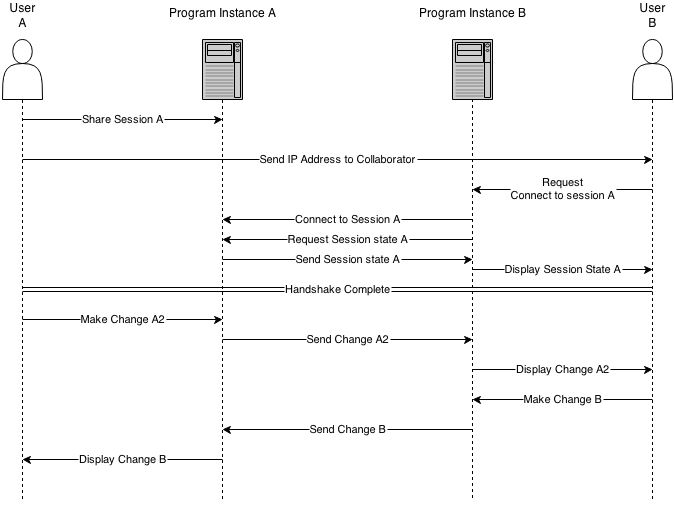
\includegraphics[width=\textwidth]{images/minf_collab_diagram.png}
    \caption{Collaboration handshake stage}
    \label{fig:collab_handshake}
\end{figure}

This approach was not without its problems.  A fundamental problem with having the collaboration follow a distributed model is how to ensure that both program instances have the same ordering of events.  Figure~\ref{fig:collab_mixup} shows this.  In this example User B makes a change before receiving the change from User A.  After both changes have been received User A will see User B's change and User B will see User A's change.  To solve this problem Lamport clocks~\cite{coularis}[p.624] were used.  tdi{Any action that affects the session state, an action that does this is one that will need to be sent to the collaborators, increments the Lamport clock -- Make this clearer}.  The Lamport clocks are then sent with every message.  When a message arrives the server checks the Lamport clock and works out where in the history it should go.  After reordering the history all the visualisations are redrawn.  This also has to be done in the instance of the program that is sending the change.  This can be seen in Figure~\ref{fig:collab_mixup_fix}.  When changes are received the history of events is reordered to ensure each user sees the same state.  User A sees User B's change and User B sees their own change.  Figure~\ref{fig:collab_mixup_fix_2} shows how using a centralised model would remove the need for reordering of events.

\tdi{Cite Lamport Clocks - Use the big book}

\begin{figure}[h!]
    \centering
    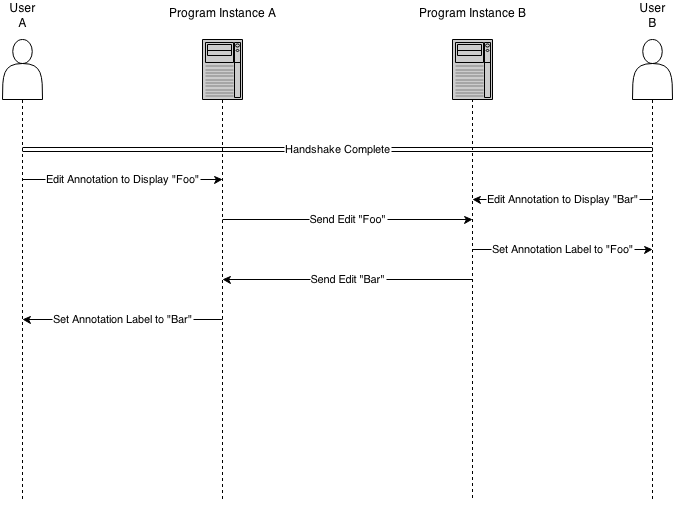
\includegraphics[width=\textwidth]{images/minf_collab_mixup.png}
    \caption{Out of sync collaboration}
    \label{fig:collab_mixup}
\end{figure}

\begin{figure}[h!]
    \centering
    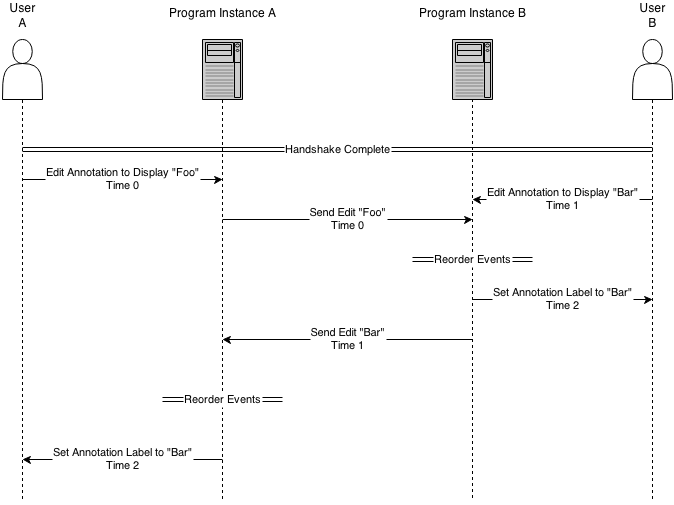
\includegraphics[width=\textwidth]{images/minf_collab_mixup_fix.png}
    \caption{Use of Lamport clocks to keep collaboration in sync}
    \label{fig:collab_mixup_fix}
\end{figure}

\begin{figure}[h!]
    \centering
    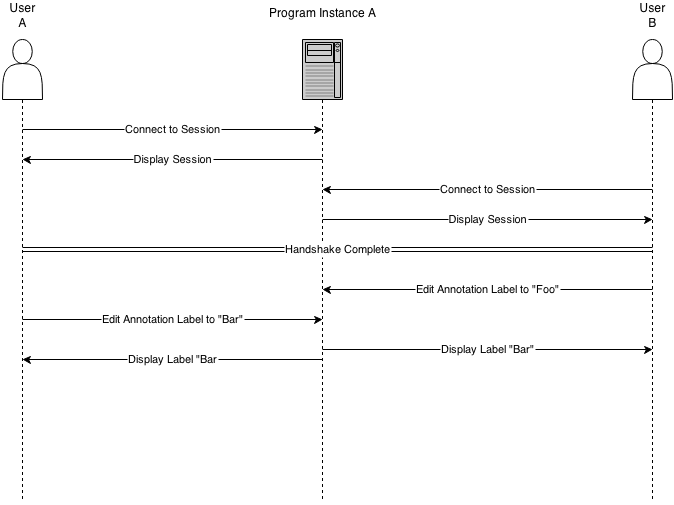
\includegraphics[width=\textwidth]{images/collaboration_single_instance.png}
    \caption{Communication flow in a centralised collaboration model.}
    \label{fig:collab_mixup_fix_2}
\end{figure}

The undo history is used to enable the event reordering.  When changes are pushed onto the undo stack they are stored as a tuple with the Lamport clock.  When a change comes in that may require events to be reordered the undo stack is searched and Lamport clocks are compared.  The new data is then inserted between the two appropriate Lamport clocks.

Another issue that was encountered was related to the initial lack of architecture.  The session data was often directly modified by methods that were bound to \ac{UI} elements: they were called when the \ac{UI} is interacted with.  These bound methods were also the methods that called the \ac{RPC} client to send the message to the collaborator. If the server on the other end then called the original bound method to perform the action it would have resulted in an infinite loop.  These methods would also often do more than just modify the state. For example when modifying an annotation the method will find the appropriate annotation and edit it.  The client would then send a message saying delete annotation 1.  The server would not be able to call the original method as it doesn't take a parameter.  The solution to this was to split the methods up more.  Now the more typical flow is the \ac{UI} bound method calling another method that modifies the state.  The server is able to call the same method.  This removes the need for duplicated code.

\section{Data Manipulation and Export}
\label{sec:normalised}

In a meeting with the developer of BioDARE it was discovered that biologists found the ability to export their data very useful.  This allows them to use their data in external applications as required.

Bio-PEPA's CSV format is non standard.  The first lines of a results file contain meta-data about the experiments.  In the worst case these lines have the potential to cause an external CSV parser to parse the data incorrectly.  In the best case the user has to delete the meta-data manually.  Allowing them to export the data, without the meta-data, makes it easier for them by removing potential errors and unnecessary steps.

Another feature that the developer of Bio-DARE recommended was allowing the biologists to normalize their data.  Biologists will often normalise their data in the y-axis.  This puts all of the data on the same scale.  This makes the data much easier to analyse if there is a significant difference in the scale.  Without it the user would be required to swap between different zoom levels.  Normalising the data makes the user's analysis much easier.

There are different normalisations that can be applied.  The data can be normalised to be zero mean and unit variance as it is for Section~\ref{sec:search}.  Another normalisation method is to normalize all the data to be between zero and one. This can be calculated using the minimum and maximum data values from the species in the results.  BioDARE allows the user to choose what type of normalisation they would like to use on their data.  For this project zero to one normalisation is the only normalisation that the user can have displayed on the graph.  This has been done to make the choice simpler for the users.  They do not have to think about which normalisation they should apply.  In the future if desired more normalisation options could be added.  Currently if they want to use a different normalisation the user can export the data and normalise that using their desired technique.

Figure~\ref{fig:annotation_intersection} shows the difference in appearance between a graph and its normalised version.

The zero to one normalised data is also exported along with the original data.  This allows the user to manipulate the normalised data in external applications if they desire.

\tdi{These last three sentences are a little lax}
